\chapter{面向初学者的拼音输入法设计}
  \section{设计初衷}

  对于中国大陆的儿童来说,初级中文教育并不会详细解释如单元音和复元音等等复杂的概念,儿童对韵母构成的理解局限于整体拼写和读音的一一对应关系。而现阶段的拼音输入法都是基于拉丁字母,对尤其是韵母部分,输入时需要进行拆分,如将 “iang” 拆分为 “i”,“a”,“n”,“g” 进行输入。这相当于要求儿童学习拉丁字母以及基于拉丁字母的键盘,对学习拼音输入的儿童来说是一种负担。

  对于国内的一些中老年人,学习中文的时候,并没有掌握学习拼音。对他们来说,复杂的拉丁字母组合也是学习拼音输入一大难题。这一部分用户使用手写输入法为主,会遇到第\ref{sec:current_input}节提到过的问题。尤其考虑到一部分半文盲用户,只具备汉语的听、说、辨识能力,还不具备正确的书写能力,学习拼音输入对他们来说更是难上加难。

  对身居海外的华侨子女,外国人来说,他们学习中文的条件和工具很有限,也是使用的笔画输入法为主。学习使用拼音输入法对他们来说很吃力,将拼音,尤其是韵母拆分为数个拉丁字母进行输入,是一种不直观而且回忆式操作门槛相对较高的方式。特别对有英文输入基础的人,QWERTY键盘反而会有一定程度上的误导性。

  本设计主要面向以上特定人群,⽬的在于克服目前技术中存在的问题,提供⼀种自然的、⾮记忆的中⽂输⼊方法,从⽽有效地减少学习负担,提高中⽂输入的效率。当然,对于已经有一定汉语基础,能够熟练掌握汉字声形的用户群体,本设计并不适用。

  此外,考虑到多点触控设备发展迅速,其尺寸有日益增大的趋势,为多点触控等交互手段提供了足够的操作空间。而目前主流拼音输入法中,并没有利用这一优势。本设计希望能充分利用大型触摸设备上多点触控的优势,同时不摒弃原来单点触控的输入方式,提供一种更灵活方便的输入体验。

  \section{设计分析}
  \subsection{布局设计}

  为了达成设计初衷,本设计采用了声母韵母分离,双通道独立输入的方式。基本输入方式与普通输入法相似,即用户通过输入设备输入目标汉字的检索信息,设备根据所属检索信息检索字库,得到候选字集并将所述字集中的汉字按顺序显示于显示屏,用户从所述候选字集选择目标汉字输入。所述检索信息包括声母和韵母两项。

  同时,本设计并没有使用拉丁字母键盘,而是根据拼音的声母和韵母,做出了一套拼音特化的键盘,分为两部分。对于每一个声母和韵母,对应键盘中都会有一个键位与之对应,并在该位置写出拉丁拼写作为标示。声母键盘和韵母键盘分别至多只能有一个键位被按下,其按下的键位的组合代表了用户想要输入的拼音。

  声母韵母的分离设计,有别于现有的QWERTY键盘和手机九键键盘,能使得输入者进行输入时,对声母韵母使用不同手进行操作。根据Kinkead等人的研究\supercite{kinkead},在进行快速打字操作的时候,当手指的操作速度达到理论最值,那么键盘布局对输入速度的影响非常之小。然而,基于人类手掌的结构,一般来说,同一只手的连续操作速度会比两只手间断操作稍慢\supercite{moscovich2008indirect}。因此,本设计将按键顺序严格限制为左右手间隔操作,意在提高用户的输入速度,与德沃夏克键盘布局将元音辅音尽量做两极化的思想类似。

  \subsection{交互设计}

  一般拼音输入法要求用户以首先输入声母,再输入韵母的方法进行输入。虽然现代拼音输入法在词组匹配,长句输入,自动纠错上做了很多贡献,但这种顺序输入的方式依然没有改变。如果在输入长句子时键入了错误的声母,就意味着需要删除到错误的点进行重新输入。由于韵母数量多于声母,如果存在有独立的两个检索通道,不要求先后的顺序关系,尤其对初学者来说,会有更多选择的余地。

  本设计考虑到了初学者的这一需求,没有强制声母和韵母的输入顺序,用户可以任意顺序输入声母和韵母,亦可在支持多点触控的平板上,同时输入声母韵母。

  考虑到声母韵母之间的搭配并非任意,而是存在一定的规则。例如,声母 “p” 与韵母 “iong” 、声母 “n” 与韵母 “ia” 等等,没有任何汉字与其读音相匹配。考虑到这种规则并没有一个清晰且容易记忆的规律,对初学者用户来说,这也是学习拼音输入的一大难点。本设计做了对初学者友好的提示设计,当声母和韵母其中一个被选中时,另一个输入区只会显示能够匹配上至少一个汉字的键位,并隐藏其他键位。例如,当韵母 “v” 被选中时,声母区只有 “l” 和 “n” 显示给用户,而其他键位都隐藏。当声母和韵母同时被选择时,则显示所有的声母和韵母键位。

  \section{具体实现}
  \subsection{整体布局}

  输入法的整体布局如图\ref{fig:layout1_background}所示。整个布局分为上下两部分。上部分为汉字显示区,会依次显示用户所输入的汉字。输入区右下角浅色的方框为拼音显示区,用于提示用户当前激活的声母以及韵母。下部分又细分为左、中、右三个子部分。左右两个子部分,分别是声母和韵母输入区,中间区域是汉字备选区。

  \begin{figure}[h]
  \noindent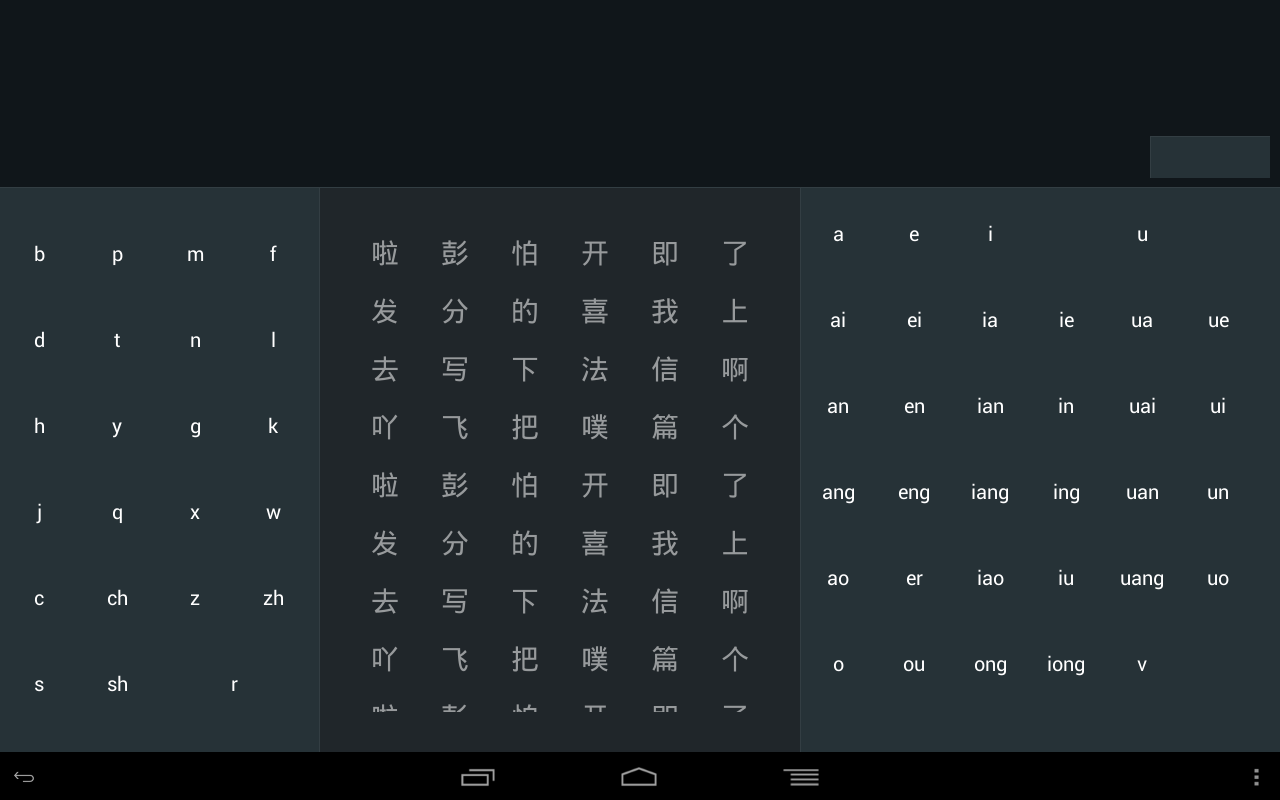
\includegraphics[width=150mm]{img/layout1_background}
  \caption{输入界面}
  \label{fig:layout1_background}
  \end{figure}

  可以看到,声母区和韵母区没有依照拉丁字母构建,完全是自定义键盘,键位涵盖了所有声母和韵母。中间部分采用大面积候选表格代替了传统的候选行,使用户能够看到更多的候选汉字。

  \subsection{输入区布局设计}

  声母输入区的键位采用了“发音部位-发音方法”的排列方法。如 ”b“、”p“ 均为双唇音,区别在于 ”b“ 是不送气音,”p“是送气音。因此,在键盘排布上,将 ”b“、”p“ 放在一行。依照“发音部位-发音方法”,将声母排列成为六行四列的表格。这种组合有两个优势:其一,使用距离远近加工了声母的近似程度,能够在初学者用户输入时给予暗示,加速其学习的速度;其二,对于不同地区的方言对声母的不区分现象主要发生在近似程度较高的声母间,输入法可以将相邻声母键位融合成一个来达到模糊输入的效果。关于对方言地区用户的输入优化在第\ref{sec:dialect}节有详细介绍。

  韵母输入区的布局思路类似声母输入区,采用”口型-元音类型“进行分类。其目的和优势都是相同的。

  声母输入区和韵母输入区均采用了无边框键位设计。根据Chaudhri等人的论述\supercite{chaudhri},目前多数虚拟键盘设计沿袭了物理键盘,采用了仿真式的视觉设计。然而,在触摸屏幕上操作,并没有实体键盘的触觉反馈,事实上只有位置信息这一个输入。这样的视觉设计是无法有效的避免误操作的。因此,本设计在视觉效果上,参考google拼音输入法\footnote{\url{https://play.google.com/store/apps/details?id=com.google.android.inputmethod.pinyin&hl=en}}采用了无边框设计。无边框设计虽然依旧无法对误操作进行改善,但能够使得整个界面看起来简单,布局明朗。

  \subsection{输入区交互设计}

  本实现包括一种过滤模块。该模块会被用户触摸屏幕事件所激活,接受并保存触摸的位置信息,并且将触摸位置映射为用户动作。具体来说,如果触摸事件位置在由于声母输入区、韵母输入区和汉字备选区,则认为此次操作是一次有效的输入操作,根据触摸位置,判断用户所希望按下的键位。其他区域的触摸事件被当做无效操作,从而忽略。对于多点触摸设备,一个输入区的多个触摸事件会产生输入冲突。在这种情况下,判断其为无效操作。而对于不支持多点触摸的设备,则不会产生冲突。

  与设计的初衷一致,当声母输入区有一个键位按下时(韵母区尚未操作),韵母区所有不能与该声母匹配的键位暂时消失,以提示用户。(见图\ref{fig:layout1_s_press_down})此时,如果用户在余下的韵母中选择了一个键位,则重新显示所有韵母输入区内容,并且在汉字备选区中加入满足该组合的所有汉字,按照使用频率降序排列。类似的,当韵母按下时,无法匹配的声母也会暂时消失。

  \begin{figure}[h]
  \noindent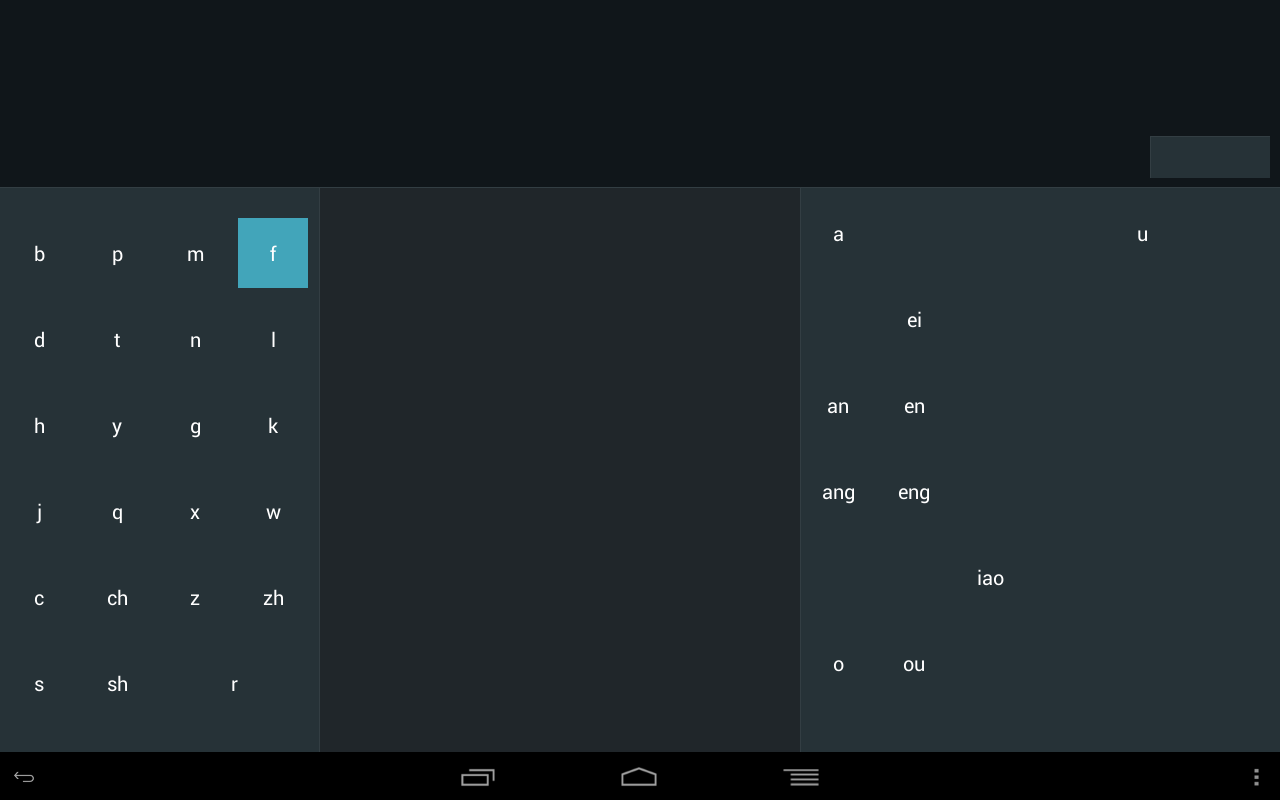
\includegraphics[width=150mm]{img/layout1_s_press_down}
  \caption{声母键位按下}
  \label{fig:layout1_s_press_down}
  \end{figure}

  当声母和韵母都有正确输入时,符合其音律组合的汉字会出现在汉字备选区中。汉字备选区采用了六列若干行的表格的形式,支持两种不同的操作:点击某一个汉字键位,表示用户选择了这一个汉字,该汉字会出现在上部汉字显示区中,并在拼音显示区显示当前输入的声母韵母组合(见图\ref{fig:layout1_finished});垂直拖动汉字备选区,表示用户希望选择的汉字没有出现在表格中,表格将上下滚动以显示更多内容。备选区选择表格这种形式,也是考虑到初学者对汉字不熟悉的情况,给予其更多汉字选择。

 % \begin{figure}[h]
 % \noindent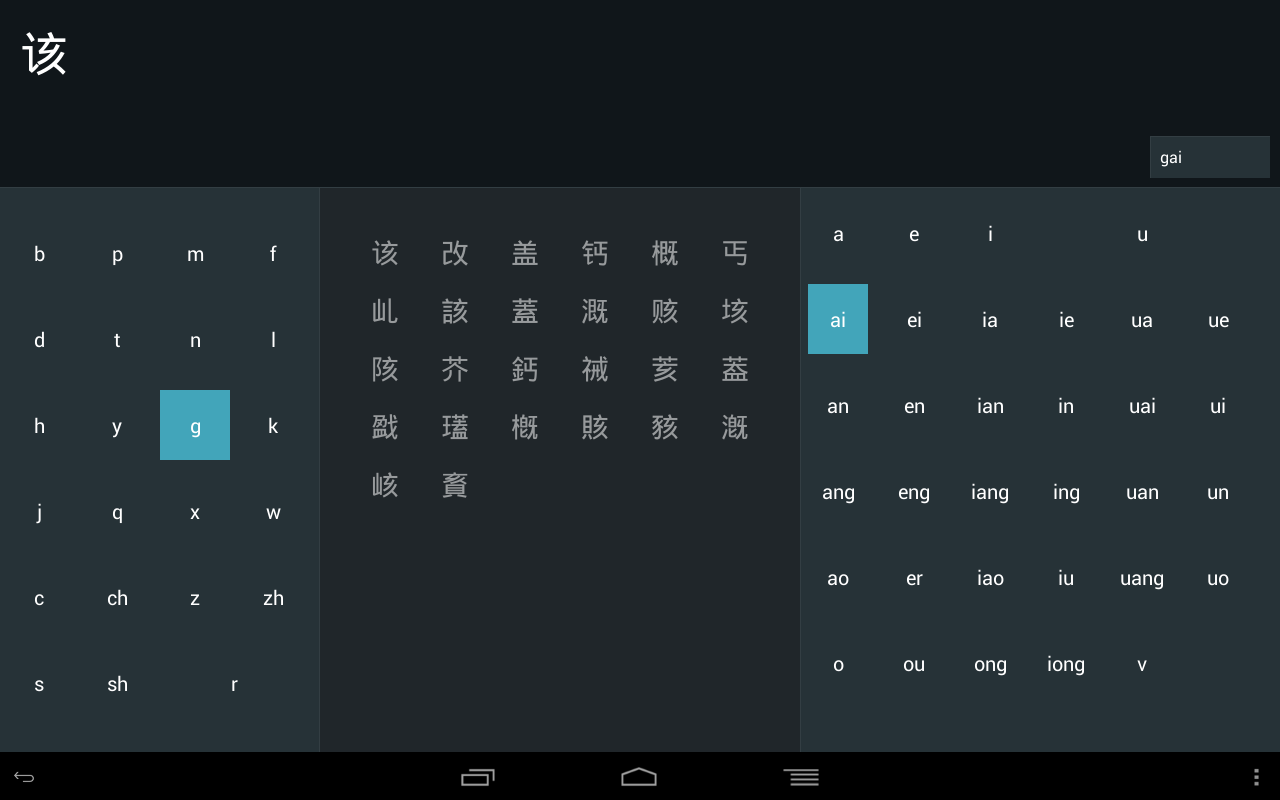
\includegraphics[width=150mm]{img/layout1_finished}
 % \caption{选择汉字操作}
 % \label{fig:layout1_finished}
 % \end{figure}

  \section{本设计的优势}

  通过与现有拼音输入法进行对比,充分考虑到第\ref{sec:limit}节所提到的现有输入法的局限性,本设计的优势有以下几点:

  \begin{enumerate}
  \item
  依托多点触摸技术,实现⾃然⽅式交互:由于该设计采用了多点触控的技术,赋予了用户更多操作的空间。例如:用户在实际操作中可以使用一个手指输入声母后保持不变,另一个手指输入韵母,双手并用,而无需像在单点触摸屏,点击后马上抬起。双⼿并用、多指操作这是最自然、最舒适的输⼊方式,符合⼤多数⼈的操作习惯,而这种自然的交互⽅式也势必是人机交互未来发展的⽅向。

  \item
  拓展多通道技术,提出韵母检索新⽅式:多通道(multi-modal,也称多模式)交互模式已被诸多研究证明是提高交互效率和自然性的有效途径。多通道交互作为未来人机交互中的一项核心技术在国内外受到了普遍的关注。\supercite{dsh,lmz}用户可以通过各种不同的交互通道以及它们之间的相互组合、协作来完成交互任务,这正好弥补了单一交互模式给用户带来的限制和负担。本设计中涉及的拼⾳声母和拼⾳韵母都以独立的显示区域存在,并且以其中任何一个作为输⼊时都可以表达⽤户的输⼊意愿,其输入内容互不相关、输出结果相互补充,在操作时具有前后⽆关性,更改其中一个的输⼊即可实现结果的修正,因此我们可以将其看作是两个独立的输⼊通道。由于拼⾳韵母是一个独⽴的输⼊通道,我们可以实现韵母的检索和提示模式,能够回避⽤户对声母混淆的问题,有效降低输入时的出错率。对于⽬前主流的单点触摸设备,本设计仍然适用。声母表区和韵母表区可以记录并保存⽤户的最后一次输入,用户可以任意顺序依次在两个区域完成输入。

  \item
  人性化设计输入界⾯面,学习记忆⽆无负担:输入界面的设计采用人体工效学的方法科学设计,具体表现为:布局合理,声母区和韵母区分别使用“发音部位-发音方法”和“口型-元音类型”的原则排列,易于用户记忆和熟练操作后提高输入速度。另外,本设计已将所有的声母、韵母以及组合完整的显示出来,用户所需的操作仅是从屏幕中罗列的拼⾳中选择⾃己认为正确组合情况,避开了繁重和易于混淆的记忆过程。

  \item
  ⽤户群体广泛,与现有输⼊法形成互补:与设计初衷一致,本设计大量考虑了拼音输入的初学者,包括学龄儿童、老人、半文盲、外国华侨及其子女等等人群,充分考量他们对学习拼音输入的困难,并从各个方面为其定制功能和外观。本发明合理的弥补了传统汉字输入法流失的⽤户群体,并与其组成了一套完整的汉字输⼊体系,能够满足所有有意愿学习和应⽤用汉语的人的要求,这势必会对汉语的普及和教育起到极大的推动作用。
  \end{enumerate}
